\section{Principal Component Analysis}

\subsection{Part 1: Comparing Principal Components}
\begin{enumerate}
    \item Report the eigenvectors and eigenvalues here. 

Eigenvectors of the dataset
\begin{itemize}
\item Eigenvector 1: $[ 0.70711,  0.70711]$
\item Eigenvector 2: $[-0.70711,  0.70711]$
\end{itemize}

Eigenvalues of the dataset
\begin{itemize}
\item 1.6530
\item 0.3583
\end{itemize}
         \item  Express mathematically, explain why the first PC is the eigenvector associated with the largest eigenvalue?
     \newline
    \item  What can you say about the relationship between the first principal component and the second?
    \newline \newline
    The two principal components are orthogonal, by construction.
\end{enumerate}

\subsection{Part 2: Plotting Principal Components in Original Space}
\begin{enumerate}
    \item Please describe how the principal components relate to the points.
\newline
\newline
    The first principal component is the direction of maximum variance whereas the second principal component is the vector orthogonal to the first in the 2D plane.
    \item Paste the graph here of the plot of the given points (with both axis in same scale) as well as the lines representing the principal components in original space, with x1 in the x axis and x2 in the y axis.
    
\begin{figure}[H]
\centering
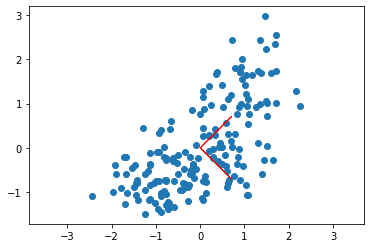
\includegraphics[width=0.7\textwidth]{templates/pca_simple}
\caption{Scatter Plot with Principal components in the original space.}
\label{fig:my_label}
\end{figure}
    
\end{enumerate}
\subsection{Part 3: Plotting Data Projected onto Component Space}
\begin{enumerate}
    \item Explain how the graph of points on principal component space relates to the graph of points on original space above.
    \newline
    \newline
    The graph of points in principal component space is simply the graph of points in the origin space, but rotated counter-clockwise by approximately $45^{\circ}$.
    \item Explain the difference in distribution of points projected on the first component vs. projected on the second.
    \newline
    \newline
    The distribution of points projected on the first component has maximal variance compared to the distribution of points projected onto the second component.        
    \item Paste the plot of the given points (with both axis in same scale) in principal component space.
    
\begin{figure}[H]
\centering
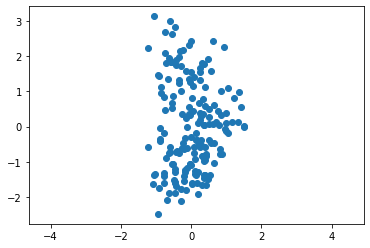
\includegraphics[width=0.7\textwidth]{templates/pca_simple_1}
\caption{Scatter plot in Principal Component space.}
\label{fig:my_label}
\end{figure}
\end{enumerate}
\subsection{Part 4: PCA and Reconstruction Error}
\begin{enumerate}
    \item Using the digit data set from the PCA worksheet (used in PCA Maximize Variance), what is the reconstruction error using the first and second principal components

\begin{figure}[H]
	\centering
	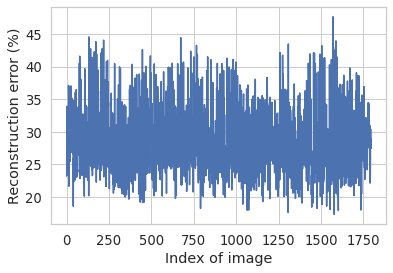
\includegraphics[width=0.5\textwidth]{templates/digit_reconstruction}
	\caption{Reconstruction error of each input image using 2 principal components.}
	\label{fig:my_label}
\end{figure}
Average reconstruction error is $28.85\%$

        \item  Mathematically express how you come up with the answer, and explain how PCA is minimizing the reconstruction error. 
        \newline \newline
Using Lagrangian multipliers, there exists $\lambda_{k+1}, \ldots, \lambda_{d}$ such that solution to above is given by:
\begin{align*}
\operatorname{min} \sum_{t=1}^{n} \sum_{j=k+1}^{d} \mathbf{w}_{j}^{\top} \Sigma \mathbf{w}_{j}+\sum_{j=k+1}^{d} \lambda_{j}\left\|\mathbf{w}_{j}\right\|_{2}^{2} & \text{\qquad $d$ is dim of the covar matrix, $K$ is number of features.}
\end{align*}        
Setting derivate to $0, \quad \Sigma \mathbf{w}_{j}=\lambda_{j} \mathbf{w}_{j} .$ That is $\mathbf{w}_{j}^{\prime} \mathrm{s}$ are eigenvectors and $\lambda_{j}$ 's are eigenvalues.
\end{enumerate}